
\subsection{Answers}
\begin{table}[htb]%
\begin{center}%
\caption{Q22: Have you ever written MPI+”X” programs? If so, select all that apply.}%
\label{tab:Q22-ans}%
\begin{tabular}{l|l|r}%
\hline%
Choice & Abbrv. & \# Answers \\%
\hline%
OpenMP & OMP & 577 (69.7\%) \\%
CUDA & CUDA & 231 (27.9\%) \\%
No & No & 190 (22.9\%) \\%
Pthread & Pthread & 155 (18.7\%) \\%
OpenACC & OACC & 79 (9.5\%) \\%
OpenCL & OCL & 43 (5.2\%) \\%
other & - & 33 (4.0\%) \\%
\hline%
\multicolumn{2}{c}{total} & 1308 (828)\\%
\hline%
\end{tabular}%
\end{center}%
\end{table}%

\clearpage%
{\footnotesize\begin{landscape}%
\begin{longtable}[htb]{r|c|c|c|c|c|c|c|c|c|c}%
\caption{Q22: Have you ever written MPI+”X” programs? If so, select all that apply.}%
\label{tab:Q22-mans} \\%
\hline%
Multi-Answer & overall & FR & GR & IT & UK & eu & JP & RU & US & others \\
 \hline%
\endfirsthead%
\multicolumn{11}{r}{(continued from the previous page)}\\%
\hline%
Multi-Answer & overall & FR & GR & IT & UK & eu & JP & RU & US & others \\
 \hline%
\endhead%
\hline%
(total) & 828 & 119 & 156 & 54 & 65 & 140 & 64 & 91 & 57 & 82 \\%
\hline%
\multicolumn{11}{r}{(continue to the next page)}\\%
\endfoot%
\hline%
(total) & 828 & 119 & 156 & 54 & 65 & 140 & 64 & 91 & 57 & 82 \\%
\hline%
\endlastfoot%
\hline%
{OMP} & 270 & 37 & 62 & 19 & 22 & 43 & 25 & 27 & 14 & 21 \\%
{No} & 190 & 24 & 41 & 19 & 13 & 28 & 8 & 25 & 5 & 27 \\%
{OMP, CUDA} & 94 & 4 & 9 & 9 & 6 & 22 & 7 & 18 & 9 & 10 \\%
{OMP, Pthread} & 60 & 14 & 13 & 1 & 11 & 7 & 4 & 2 & 5 & 3 \\%
{OMP, Pthread, CUDA} & 36 & 5 & 9 & 0 & 1 & 4 & 4 & 4 & 6 & 3 \\%
{OMP, OACC} & 24 & 6 & 2 & 1 & 2 & 7 & 3 & 0 & 0 & 3 \\%
{OMP, OACC, CUDA} & 21 & 3 & 4 & 0 & 1 & 3 & 4 & 0 & 3 & 3 \\%
{CUDA} & 19 & 1 & 0 & 0 & 2 & 4 & 2 & 5 & 3 & 2 \\%
{Pthread} & 16 & 4 & 0 & 1 & 2 & 2 & 0 & 3 & 3 & 1 \\%
{OMP, OCL, CUDA} & 14 & 4 & 0 & 1 & 0 & 5 & 0 & 2 & 2 & 0 \\%
{OMP, Pthread, OACC, CUDA} & 9 & 1 & 1 & 0 & 1 & 0 & 3 & 0 & 1 & 2 \\%
{OMP, Pthread, OCL, CUDA} & 7 & 1 & 2 & 1 & 0 & 1 & 0 & 0 & 1 & 1 \\%
{OMP, OACC, OCL, CUDA} & 5 & 0 & 1 & 1 & 0 & 2 & 0 & 0 & 1 & 0 \\%
{Pthread, CUDA} & 5 & 2 & 0 & 0 & 0 & 2 & 0 & 1 & 0 & 0 \\%
{OMP, Pthread, OACC, OCL, CUDA} & 4 & 0 & 1 & 1 & 0 & 1 & 1 & 0 & 0 & 0 \\%
{OMP, Pthread, OACC} & 3 & 0 & 1 & 0 & 1 & 0 & 1 & 0 & 0 & 0 \\%
{OCL} & 3 & 1 & 0 & 0 & 0 & 0 & 0 & 1 & 0 & 1 \\%
{Pthread, OACC} & 2 & 1 & 0 & 0 & 0 & 0 & 0 & 0 & 0 & 1 \\%
{OMP, TBB} & 2 & 0 & 1 & 0 & 0 & 0 & 0 & 0 & 1 & 0 \\%
{Pthread, OCL, CUDA} & 2 & 0 & 0 & 0 & 0 & 1 & 0 & 1 & 0 & 0 \\%
{OACC} & 2 & 0 & 0 & 0 & 1 & 1 & 0 & 0 & 0 & 0 \\%
{OACC, CUDA} & 2 & 1 & 0 & 0 & 0 & 1 & 0 & 0 & 0 & 0 \\%
{OMP, OACC, OCL} & 2 & 0 & 1 & 0 & 0 & 0 & 0 & 0 & 1 & 0 \\%
{OMP, GASPI} & 2 & 0 & 2 & 0 & 0 & 0 & 0 & 0 & 0 & 0 \\%
{OCL, CUDA} & 2 & 1 & 0 & 0 & 0 & 1 & 0 & 0 & 0 & 0 \\%
{OMP, Pthread, OCL} & 2 & 2 & 0 & 0 & 0 & 0 & 0 & 0 & 0 & 0 \\%
{OMP, Pthread, Cilk++} & 1 & 1 & 0 & 0 & 0 & 0 & 0 & 0 & 0 & 0 \\%
{OMP, coupling applications implemented in various languages (C++, fortran, Python) with MPI} & 1 & 1 & 0 & 0 & 0 & 0 & 0 & 0 & 0 & 0 \\%
{OMP, MPI-3 shared memory windows} & 1 & 0 & 1 & 0 & 0 & 0 & 0 & 0 & 0 & 0 \\%
{OMP, CUDA, Python} & 1 & 0 & 0 & 0 & 0 & 0 & 0 & 1 & 0 & 0 \\%
{OMP, Pthread, StarPU} & 1 & 1 & 0 & 0 & 0 & 0 & 0 & 0 & 0 & 0 \\%
{OMP, Pthread, OACC, CUDA, TBB, C++11 threads.} & 1 & 0 & 0 & 0 & 0 & 1 & 0 & 0 & 0 & 0 \\%
{CUDA, StarPU, Intel TBB, MassiveThreads} & 1 & 0 & 0 & 0 & 0 & 0 & 1 & 0 & 0 & 0 \\%
{OMP, Pthread, MPI + Pthread but only via library (PaStiX)} & 1 & 0 & 1 & 0 & 0 & 0 & 0 & 0 & 0 & 0 \\%
{Sunway athread} & 1 & 0 & 0 & 0 & 0 & 0 & 0 & 0 & 0 & 1 \\%
{OMP, Pthread, OCL, CUDA, C++ threads} & 1 & 0 & 0 & 0 & 0 & 1 & 0 & 0 & 0 & 0 \\%
{OMP, OACC, TBB} & 1 & 0 & 0 & 0 & 1 & 0 & 0 & 0 & 0 & 0 \\%
{OMP, Pthread, OmpSs} & 1 & 0 & 1 & 0 & 0 & 0 & 0 & 0 & 0 & 0 \\%
{OMP, CUDA, MPI + MPI} & 1 & 0 & 0 & 0 & 1 & 0 & 0 & 0 & 0 & 0 \\%
{OMP, tbb GASPI} & 1 & 1 & 0 & 0 & 0 & 0 & 0 & 0 & 0 & 0 \\%
{OMP, CUDA, kokkos} & 1 & 1 & 0 & 0 & 0 & 0 & 0 & 0 & 0 & 0 \\%
{OMP, Pthread, CUDA, Tbb} & 1 & 1 & 0 & 0 & 0 & 0 & 0 & 0 & 0 & 0 \\%
{Julia GPU} & 1 & 0 & 0 & 0 & 0 & 0 & 0 & 0 & 1 & 0 \\%
{OMP, OACC, ompss} & 1 & 1 & 0 & 0 & 0 & 0 & 0 & 0 & 0 & 0 \\%
{Pthread, UPC, UPC++} & 1 & 0 & 0 & 0 & 0 & 0 & 0 & 0 & 1 & 0 \\%
{Sunway Athread, OACC} & 1 & 0 & 0 & 0 & 0 & 0 & 0 & 0 & 0 & 1 \\%
{OMP, OCL} & 1 & 0 & 1 & 0 & 0 & 0 & 0 & 0 & 0 & 0 \\%
{athread} & 1 & 0 & 0 & 0 & 0 & 0 & 0 & 0 & 0 & 1 \\%
{OMP, CUDA, Intel TBB} & 1 & 0 & 1 & 0 & 0 & 0 & 0 & 0 & 0 & 0 \\%
{Pthread, TensorFlow} & 1 & 0 & 0 & 0 & 0 & 0 & 1 & 0 & 0 & 0 \\%
{OMP, Just as exercise in classes, or seen in others' programs} & 1 & 0 & 0 & 0 & 0 & 1 & 0 & 0 & 0 & 0 \\%
{OMP, OACC, CUDA, CUDA Fortran} & 1 & 0 & 0 & 0 & 0 & 1 & 0 & 0 & 0 & 0 \\%
{OMP, Kokkos} & 1 & 0 & 0 & 0 & 0 & 0 & 0 & 0 & 0 & 1 \\%
{OMP, ("MPI + MPI-3 shared memory" instead of "MPI+OpenMP")} & 1 & 0 & 1 & 0 & 0 & 0 & 0 & 0 & 0 & 0 \\%
{CUDA, Posix ShM} & 1 & 0 & 0 & 0 & 0 & 0 & 0 & 1 & 0 & 0 \\%
{OMP, CUDA, ROCm} & 1 & 0 & 0 & 0 & 0 & 1 & 0 & 0 & 0 & 0 \\%
\hline%
\end{longtable}%
\end{landscape}}%
\clearpage%


\subsection{List of other answers}
\begin{itemize}
\item China: Sunway Athread
\item China: Sunway athread
\item China: athread
\item Europe:France: Cilk++
\item Europe:France: StarPU
\item Europe:France: Tbb
\item Europe:France: coupling applications implemented in various languages (C++, fortran, Python) with MPI
\item Europe:France: kokkos
\item Europe:France: ompss
\item Europe:France: tbb GASPI
\item Europe:Germany: ("MPI + MPI-3 shared memory" instead of "MPI+OpenMP")
\item Europe:Germany: GASPI
\item Europe:Germany: GASPI
\item Europe:Germany: Intel TBB
\item Europe:Germany: MPI + Pthread but only via library (PaStiX)
\item Europe:Germany: MPI-3 shared memory windows
\item Europe:Germany: OmpSs
\item Europe:Germany: TBB
\item Europe:UK: MPI + MPI
\item Europe:UK: TBB
\item Europe:others: C++ threads
\item Europe:others: CUDA Fortran
\item Europe:others: Just as exercise in classes, or seen in others' programs
\item Europe:others: ROCm
\item Europe:others: TBB, C++11 threads.
\item Japan: StarPU, Intel TBB, MassiveThreads
\item Japan: TensorFlow
\item Russia: Posix ShM
\item Russia: Python
\item South Korea: Kokkos
\item USA: Julia GPU
\item USA: TBB
\item USA: UPC, UPC++

\end{itemize}
This questions relates on how hybrid programming is common within the
developers. 

Only a small fraction (15\%) of the developers have never written an MPI  program
without any other parallel programming language/model. The language
or API the most used with MPI is OpenMP (44\%) followed by CUDA
(17\%). This seems required to manage multicore or accelerator-based parallel
system. 

\begin{figure}[htb]
\begin{center}
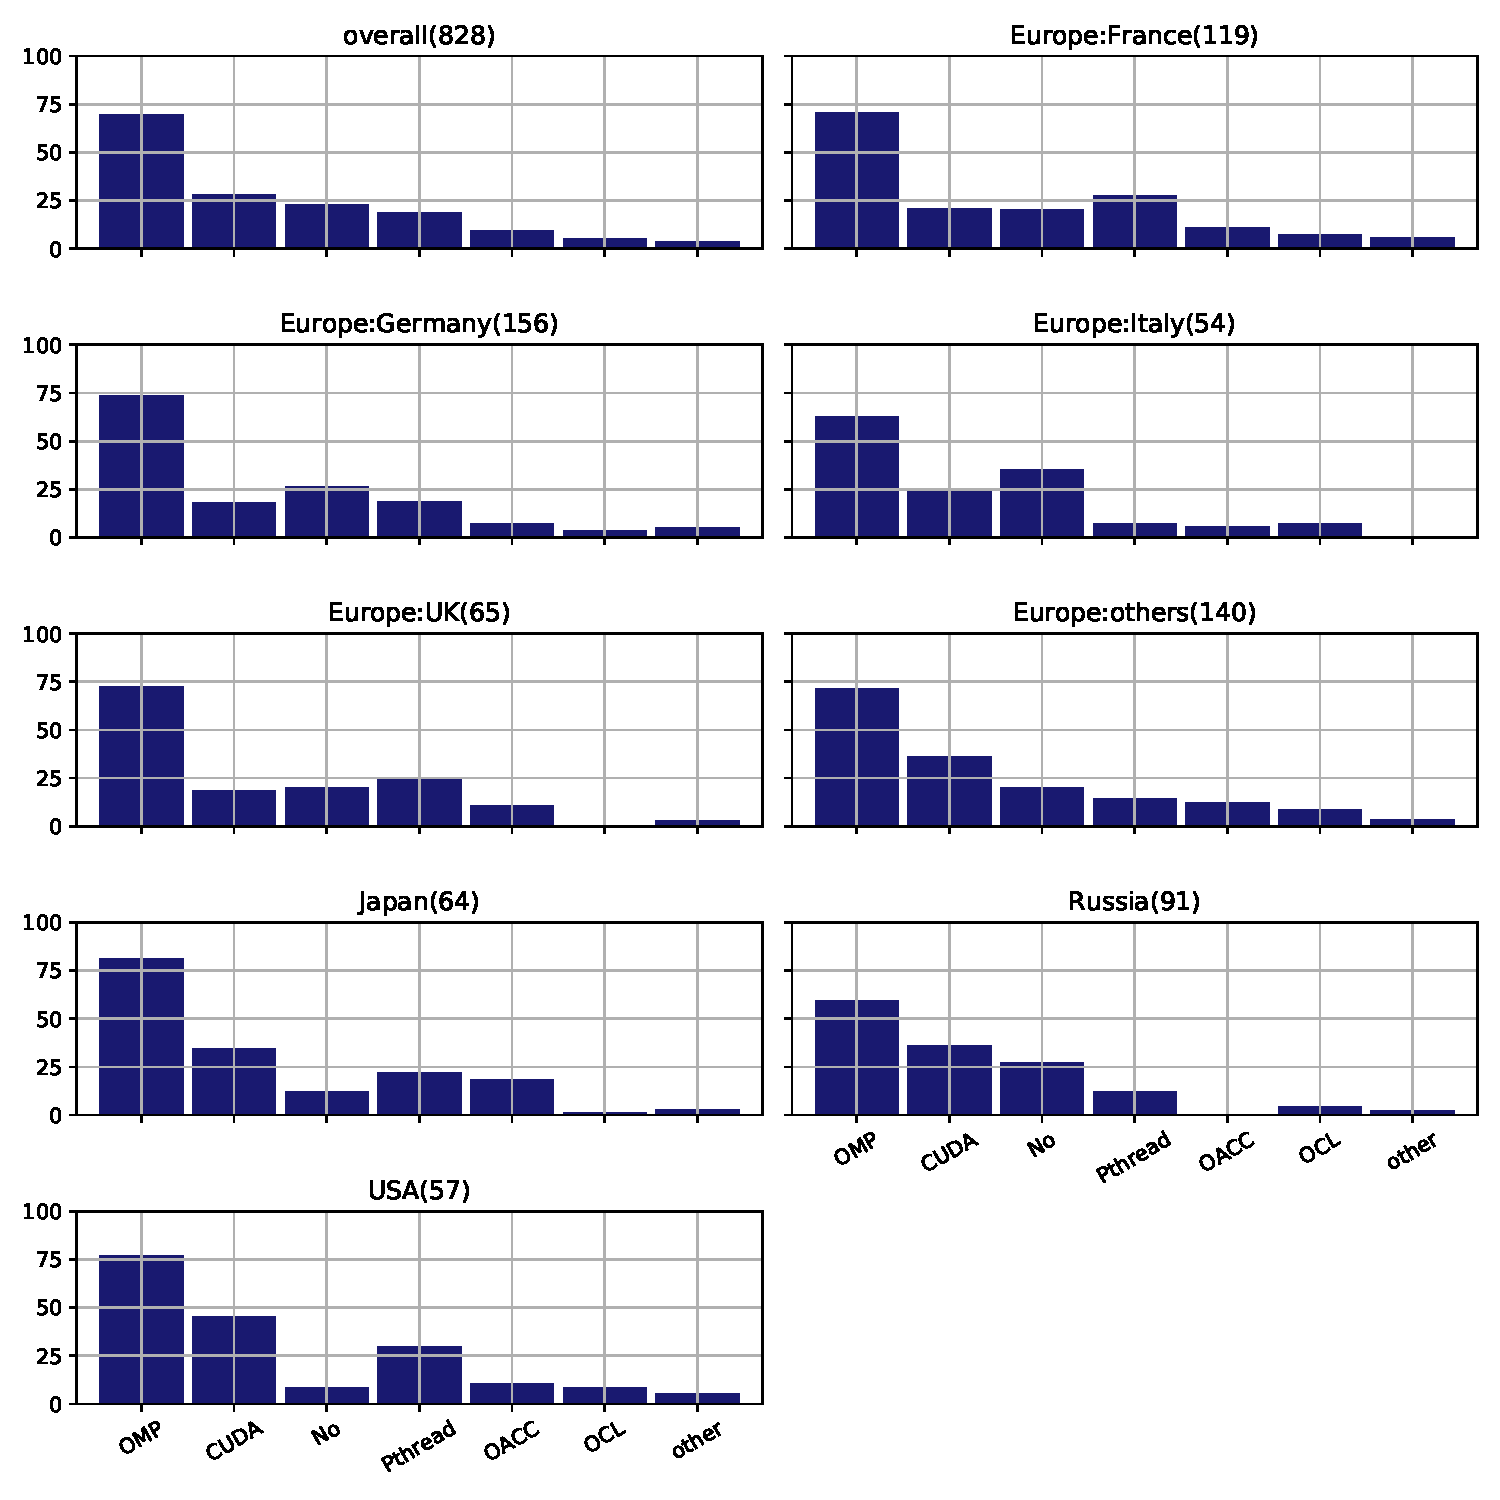
\includegraphics[width=10cm]{../pdfs/Q22.pdf}
\caption{Simple analysis: Q22}
\label{fig:Q22}
\end{center}
\end{figure}

In general, around 40\% of all countries/regions of MPI users
use MPI with OpenMP. The hybrid technique is very common.
It is interesting that the percentage of 'no' answer in US is the
smallest. 
